\vspace{-1cm}
\begin{wrapfigure}{r}{5cm}
  \centering
  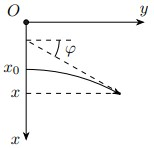
\includegraphics[width=0.25\textwidth]{Figures/Fig 5S1.jpg}
\end{wrapfigure}

\noindent\textbf{1.} Vì chùm sáng chiếu tới theo phương pháp tuyến nên nó không bị khúc xạ khi đi vào lăng kính. Gọi $\varphi$ là góc hợp bởi tiếp tuyến của quỹ đạo tia sáng tại điểm đang xét với trục $Oy$, $x_{0}$ là toạ độ mà tia sáng đi vào. Từ định luật Snell, ta có:
\begin{equation*}
  n\cos\varphi=\frac{3\cos\varphi}{2-\dfrac{x}{h}}=\frac{3}{2-\dfrac{x_{0}}{h}}\implies\cos\varphi=\frac{2h-x}{2h-x_{0}}
\end{equation*}
lấy vi phân hai vế ta được:
\begin{equation*}
  dx=\left(2h-x_{0}\right)\sin\varphi d\varphi
\end{equation*}
bên cạnh đó:
\begin{equation*}
  \tan\varphi=\frac{dx}{dy}
\end{equation*}
suy ra:
\begin{equation*}
  dy=dx\cot\varphi=(2h-x_{0})\cot\varphi\sin\varphi d\varphi=(2h-x_{0})\cos\varphi d\varphi
\end{equation*}
tại $y=0$ thì $\varphi=0$, do đó:
\begin{equation*}
  y(\varphi)=(2h-x_{0})\int_{0}^{\varphi}\cos\varphi d\varphi=(2h-x_{0})\sin\varphi
\end{equation*}
vì:
\begin{equation*}
  1=\sin^{2}\varphi+\cos^{2}\varphi=\left(\frac{y}{2h-x_{0}}\right)^{2}+\left(\frac{x-2h}{2h-x_{0}}\right)^{2}
\end{equation*}
nên:
\begin{equation*}
  y^{2}+(x-2h)^{2}=(2h-x_{0})^{2}
\end{equation*}

\newpage
\begin{wrapfigure}{r}{6.5cm}
  \centering
  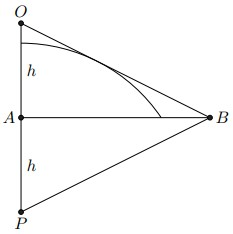
\includegraphics[width=0.35\textwidth]{Figures/Fig 5S2.jpg}
\end{wrapfigure}

\noindent\textbf{2.} Từ kết quả của ý trên, ta nhận thấy rằng quỹ đạo của bất kỳ tia sáng nào bên trong lăng kính, trước khi đi đến các mặt $AB$ và $OB$, đều là các cung tròn có tâm $P$ nằm tại điểm có toạ độ $(x_{P},y_{P})$, với $x_{P}=2h$ và $y_{P}=0$. Bán kính của các cung tròn giảm dần khi toạ độ $x_{0}$ tăng lên. Khoảng cách từ điểm $P$ đến giao điểm của cung tròn với $OB$ sẽ giảm dần cho đến khi cung tròn chạm tới cạnh đang xét. Khi toạ độ $x_{0}$ tiếp tục tăng, các cung tròn sẽ không còn đi qua cạnh $OB$. Do đó, để các tia chạm đến mọi điểm trên mặt $OB$, góc $\hat{PBO}$ không được là góc nhọn, vì tam giác $OPB$ là tâm giác cân, ta có:
\begin{equation*}
  \hat{PBO}=180^{\circ}-2\alpha\geqslant 90^{\circ}\implies\alpha\leqslant 45^{\circ}
\end{equation*}

\begin{wrapfigure}{r}{6.5cm}
  \centering
  \vspace{-1cm}
  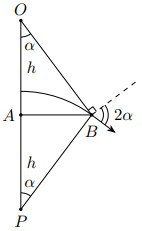
\includegraphics[width=0.25\textwidth]{Figures/Fig 5S3.jpg}
\end{wrapfigure}

\noindent\textbf{3.} Khi toạ độ $x_{0}$ tăng lên, góc tới của các tia sáng trên mặt bên $OB$ sẽ tăng. Để các tia sáng đi đến $OB$ đều khúc xạ ra bên ngoài, hiện tượng phản xạ toàn phần không được xảy ra. Vì ban đầu góc tới của các tia sáng so với $OB$ là $\alpha$, sau khi chúng di chuyển theo cung tròn, góc tới này sẽ bị quay một góc $\alpha$, như vậy, góc tới của các tia sáng khi chiếu đến mặt bên $OB$ là $2\alpha$. Ta có:
\begin{equation*}
  n(h)\sin 2\alpha=3\sin 2\alpha\geqslant 1\implies \alpha\leqslant\frac{1}{2}\arcsin\frac{1}{3}\approx9,74^{\circ}
\end{equation*}
